\documentclass[usenames,dvipsnames]{standalone}
\usepackage{tikz}
\usepackage{tikz-network}
\usepackage{libertine}
\usepackage{libertinust1math}
\usepackage{pgfplots}

\usepackage[T1]{fontenc}
\usetikzlibrary{patterns.meta,decorations.pathmorphing}

\begin{document}
	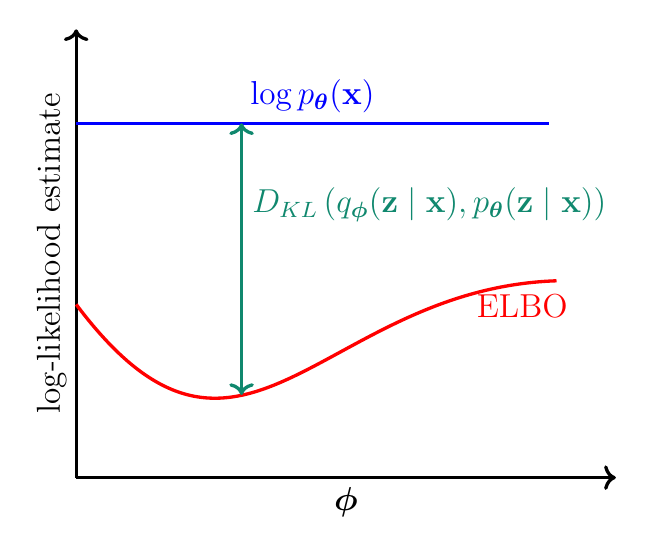
\begin{tikzpicture}
		\begin{axis}[xmin=0,xmax=100,ymin=0,ymax=4.5,
			axis line style = very thick,
			xmajorticks=false,
			ymajorticks=false,
			axis lines=middle,
			axis line style={->},
			x label style={at={(axis description cs:0.5,0.0)},anchor=north},
			y label style={at={(axis description cs:0.0,.5)},rotate=90,anchor=south},
			ylabel={\large log-likelihood estimate},
			xlabel={\large $\boldsymbol{\phi}$}]
		\end{axis}
				
		\draw[very thick, blue] (0,4.5)  -- node[midway, above] {\large $\log p_{\boldsymbol{\theta}}(\mathbf{x})$}  (6,4.5);
		\draw[very thick, red] (0.0,2.2) .. controls (2.1,-0.6) and (3.1,2.4) .. (6.1,2.5) node[below, pos=.95]{\large ELBO};

		\draw[<->, very thick, color=PineGreen] (2.1, 4.5) -- (2.1, 1.05) node[color=PineGreen, right, pos=.3] {\large $D_{K L}\left(q_{\boldsymbol{\phi}}(\mathbf{z} \mid \mathbf{x}), p_{\boldsymbol{\theta}}(\mathbf{z} \mid \mathbf{x})\right)$};

\end{tikzpicture}
\end{document}